\chapter{Grundlagen}

Im folgenden Kapitel sollen konzeptionelle Grundlagen erläutert werden, welche für das Verständnis der Bachelorarbeit notwendig sind.
Dabei wird auf die Themen Requirements Engineering, Augmented Reality und die Software reQlab eingegangen.

  \section{Requirements Engineering}
  Die Bachelorarbeit soll sogenannte Requirements, also Anforderungen, visualisieren.
  Daher ist es für das Verständnis der Arbeit wichtig, die Grundlagen des Requirements Engineering zu kennen.

    \titleemph{Requirements}

    Grundlegend sind Requirements Anforderungen, die an ein System gestellt werden.
    Das International Requirements Engineering Board (IREB) definiert sie in ihrem Glossar mit drei Eigenschaften:
    \begin{itemize}
        \item Ein Bedürfnis eines Interesseneigners (Stakeholder).
        \item Eine Eigenschaft oder Fähigkeit, die ein System haben soll.
        \item Eine dokumentierte Repräsentation eines Bedürfnisses, einer Fähigkeit oder einer Eigenschaft.
    \end{itemize}
    \autocite[][Def. Anforderung]{ireb_cpre_glossary}

    Sie sollen also die Bedürfnisse der Stakeholder an das System repräsentieren und dokumentieren.

    Die Gestaltung von Requirements kann dabei je nach System und Anforderungen unterschiedlich sein. Chris Rupp nennt in ihrem Buch \glqq{}Requirements-Engineering und -Management\grqq{} einige Beispiele für verschiedene Formen für Requirements:
    \begin{itemize}
        \item User-Stories
        \item Use-Cases
        \item Stories
        \item formalisierte natürlichsprachliche Anforderungen
        \item Anforderungen in Form von Diagrammen (semiformales Modell)
    \end{itemize}
    \autocite[][S. 19]{Rupp2014}

    
    Natürlichsprachliche Anforderungen können sehr einfach selbst formuliert werden, sind dadurch jedoch auch anfällig für Missverständnisse und Unklarheiten.
    Das Ziel von reQlab ist es, diese Missverständnisse und Unklarheiten zu erkennen und so die Qualität der Anforderungen zu verbessern.
    Daher werden im Unfamg dieser Bachelorarbeit nur natürlichsprachliche Anforderungen genutzt.

    Zudem werden Requirements in funktionale und nicht-funktionale Requirements unterteilt.
    Funktionale Requirements beschreiben \glqq{}die Funktionen, die das System leisten soll, die Informationen die es verarbeiten soll; das gewünschte Verhalten, welches das System an den Tag legen soll.\grqq{} \autocite[][S. 12]{Hruschka2023}
    Nicht-funktionale Requirements hingegen beschreiben alle Requirements, die nicht funktionaler Natur sind, also beispielsweise Performance, Sicherheit oder Zuverlässigkeit.
    Peter Hruschka beschreibt in seinem Buch Funktionale Anforderungen mit der Frage: \glqq{}Was soll das System/Produkt tun?\grqq{}.
    Auch unterteilt er nicht-funktionale Anforderungen in die zwei Kategorien Qualitätsanforderungen (\glqq{}Wie gut? Wie schnell? Wie zuverlässig? ...\grqq{}) und Randbedingungen (\glqq{}Ressourcen, Wiederverwendung, Zukauf, geforderte Technologie ...\grqq{}) \grqq{} \autocite[][S. 13]{Hruschka2023}.
    Diese Unterteilung ist hilfreich zur Strukturierung der Anforderungen und könnte im User-Interface der Visualisierung genutzt werden, um die Anforderungen zu kategorisieren.
    
    \titleemph{Stakeholder}

    Stakeholder können \glqq{}Personen oder Organisationen sein, die die Anforderungen eines Systems beeinflussen oder die von dem System beeinflusst werden.\grqq{} \autocite[][]{ireb_cpre_glossary}.
    Beispielsweise wären die Endnutzer eines Systems Stakeholder, welche durch das System beeinflusst werden.
    Sie haben also ein Bedürfnis an das System, können dieses jedoch nicht selbst umsetzen.
    Im Gegensatz dazu stehen die Auftraggeber beziehungsweise der Produkteigner (Product Owner), welche das System entwickeln und die Anforderungen festlegen.

    Je nach der Größe und Komplexität des Systems kann es sehr viele Anforderungen geben.
    Durch die Menge an Anforderungen kann so schnell die Übersicht über das System und dessen Requirements verloren gehen, vor allem für Stakeholder, die nicht tagtäglich mit dem System arbeiten.

    \titleemph{System}

    Die IREB definiert ein System als \glqq{}Eine kohärente, abgrenzbare Menge von Elementen, die durch koordiniertes Handeln einen bestimmten Zweck erfüllen.\grqq{} \autocite[][]{ireb_cpre_glossary}
    Das Wort System ist dabei ein Überbegriff für Produkte, Services, Geräte, Prozeduren und Werkzeuge und kann sowohl physisch als auch virtuell sein.
    Daher wird auch in dieser Bachelorarbeit das Wort System als Überbegriff für alle Arten von Systemen genutzt.

    \titleemph{Requirements Engineering}

    Requirements-Engineering ist der Prozess, in dem Anforderungen an ein System erhoben, dokumentiert, analysiert, spezifiziert und validiert werden.
    Laut Chris Rupp besteht Requirements-Engineering dabei aus vier Haupttätigkeiten:
    \begin{itemize}
        \item Wissen vermitteln
        \item Gute Anforderungen herleiten
        \item Anforderungen vermitteln
        \item Anforderungen verwalten
    \end{itemize}
    \autocite[][S.20]{Rupp2014}

    Diese Bachelorarbeit soll versuchen einen neuen Ansatz in der Vermittlung von Anforderungen zu finden, um so langfristig die Qualität und Nützlichkeit der Anforderungen zu verbessern.
    Zudem soll die Visualisierung der Anforderungen helfen, bei großen Projekten die eine sehr große Zahl an Anforderungen besitzen, eine Übersicht über die Anforderungen zu erhalten und so eventuell eine bessere Kommunikation zwischen Stakeholdern und Entwicklern zu ermöglichen.

  \section{reQlab}

  Die Software reQlab ist ein Requirements-Engineering-Tool, welches von der IT-Designers GmbH entwickelt wird.
  Es dient dazu, Requirements automatisiert zu analysieren und zu bewerten.
  Dafür nutzt die Software ein Large-Language-Model (LLM), welches natürlichsprachliche Anforderungen analysiert und bewertet.
  Daher werden in reQlab alle Anforderungen als natürlichsprachliche Anforderungen verfasst um dann vom LLM verarbeitet werden zu können.
  Die Software analysiert diese Anforderungen und gibt eine begründete Bewertung aus, ob die Anforderung gut oder schlecht ist und gibt Verbesserungsvorschläge.
  Das Ziel von reQlab ist es, die Qualität der Anforderungen zu verbessern und so die Qualität des gesamten Systems zu steigern.


  \section{Virtuelle Realität}
  Für das Verständnis von Augmented Reality ist es wichtig, die Begriffe der virtuellen Realität zu kennen und zu verstehen.
  Dabei wird der Nutzer in eine virtuelle Welt versetzt, die durch Computer generiert wird.
  In virtueller Realität ist, im Gegensatz zu Augmented Reality die gesamte Umgebung digital.
  \autocite[vgl.][S.15]{Dalton2023}
  Zusätzlich wird unterschieden zwischen immersiver und nicht-immersiver virtueller Realität.
  Folgende auf den Nutzer bezogene Eigenschaften sind dabei Indikatoren für nicht-immersive virtuelle Realität:
  \begin{itemize}
    \item Der Nutzer steht nicht im Mittelpunkt.
    \item Der Nutzer ist nicht vollständig von digitalen Inhalten umgeben.
    \item Der Nutzer erfährt die virtuelle Realität als Beobachter anstatt als Teilnehmer.
  \end{itemize}
  Bei immersiver virtueller Realität sind alle äußeren Einflüsse so weit reduziert wie möglich und alle Indikatoren sollten auf immersive virtuelle Realität hinweisen.
  Der Nutzer sollte bei immersiver VR das Gefühl haben, sich selbst in der virtuellen Umgebung zu befinden.
  \autocite[vgl.][S.23-24]{Wolfel2023}

  \section{Augmented Reality}
  Augmented Reality (AR) ist eine Technologie, die die reale Welt mit digitalen Informationen erweitert.
  Dabei wird ein ähnlicher Ansatz wie bei Virtueller Realität verfolgt, jedoch wird die reale Welt nicht komplett ersetzt, sondern nur erweitert.
  Der Nutzer sieht also weiterhin seine reale Umgebung, diese wird aber durch digitale Informationen ergänzt.
  \begin{figure}[H]
    \centering
    
\includegraphics[width=0.9\textwidth]{images/RV-Continuum.png}
    \caption{Realitäts-Virtualitäts-Kontinuum nach Milgram}
    \label{fig:rv-continuum}
  \end{figure}
  Auf dem Realitäts-Virtualitäts-Kontinuum von Milgram, welches, wie in Abbildung \ref{fig:rv-continuum} dargestellt, einen fließenden Übergang zwischen Realität und Virtualität beschreibt, liegt Augmented Reality zwischen der realen Welt und der virtuellen Welt \autocite[vgl.][S.9]{milgram1999}.
  Daher fällt Augmented Reality unter den Überbegriff der Mixed Reality, da die reale Welt mit der digitalen Welt gemischt wird.
  Für diese Erweiterung der Realität müssen die Anzeigegeräte auch Informationen über die echte Umgebung sammeln können.
  Will man beispielsweise virtuelle Objekte in die reale Welt einfügen, so muss das Anzeigegerät die eigene Position kontinuierlich bestimmen können und die Position und Rotation des virtuellen Objekts anhand der Bewegungen des Nutzers anpassen.

  Anzeigegeräte für Augmented Reality haben viele Gemeinsamkeiten mit Anzeigegeräten für Virtuelle Realität.
  Die Besonderheit von AR-Anzeigegeräten ist jedoch, dass sie die reale Welt mit digitalen Informationen erweitern.
  Das heißt sie müssen dem Nutzer auch eine Sicht auf die reale Welt ermöglichen und in diese Informationen einblenden.
  Beispielsweise kann das Display eines Anzeigegeräts transparent sein, sodass der Nutzer durch das Display hindurch sehen kann, oder das Gerät kann eine Kamera haben, dessen Aufnahme auf undurchsichtige Bildschirme projiziert wird.
  Dafür gibt es verschiedene Arten von Anzeigegeräten, die für Augmented Reality genutzt werden können, wobei man allgemein zwischen 3 Haputkategorien unterscheiden kann: Head-Mounted Displays, Hand-Held-Devices und Spatial Displays \autocite[][S. 346]{Carmigniani2011}.
  Im Folgenden werden einige dieser Anzeigegeräte erklärt und ihre Use-Cases erläutert.

  \subsection{Head-Mounted Displays}
    Head-Mounted Displays (HMDs) sind grundsätzlich Bildschirme, die direkt auf dem Kopf des Nutzers getragen werden.
    Durch ihre Nähe zu den Augen des Nutzers können sie ein großes Sichtfeld abdecken, ohne dabei selbst große Displays zu nutzen.
    Dadurch sind sie für volle Immersion im Normalfall kosteneffektiver als große Displays, wie bspw. eine Leinwand.


    \subsubsection{VR Headsets}

    Klassische VR-Headsets kann man sich vorstellen wie eine Skibrille mit 2 Bildschirmen, die auf dem Kopf getragen wird und üblicherweise 2 Displays hinter 2 Linsen hat, bzw. ein Display virtuell in 2 Displays aufteilt.
    Durch die 2 Bildschirme wird für jedes Auge ein eigenes Bild erzeugt, wodurch Inhalte in 3D dargestellt werden können.
    Außerdem können sie das volle Sichtfeld des Nutzers abdecken und so eine immersive Erfahrung schaffen.

    Die Position des Headsets muss dabei kontinuierlich bestimmt werden, um die Bewegungen der Nutzer zu verfolgen und so die virtuelle Welt anpassen zu können.
    Dies geschieht meist durch Basisstationen (bspw. bei der Valve Index) oder durch Kameras im Headset (bspw. bei der Oculus Quest 3).
    Die Interaktion mit der Umgebung wird dann meist mit Controllern realisiert, deren Position und Rotation ebenfalls kontinuierlich bestimmt werden muss.
    In VR-Headsets mit eigenen Kameras ist es auch möglich, die Hände des Nutzers zu tracken und als Controller zu nutzen.
    Dabei können dann bestimmte Gesten oder Handbewegungen als Eingabe interpretiert werden.
    
    Ursprünglich mussten VR-Headsets mit einem Computer verbunden werden, um die Rechenleistung für die Darstellung der Inhalte zu haben.
    Mit der Zeit wurden jedoch auch standalone VR-Headsets, wie bspw. die 2024 auf den Markt gebrachte Apple Vision Pro, die ihre eigene Rechenleistung haben und so unabhängig von einem Computer genutzt werden können.

    \begin{figure}[H]
      \centering
      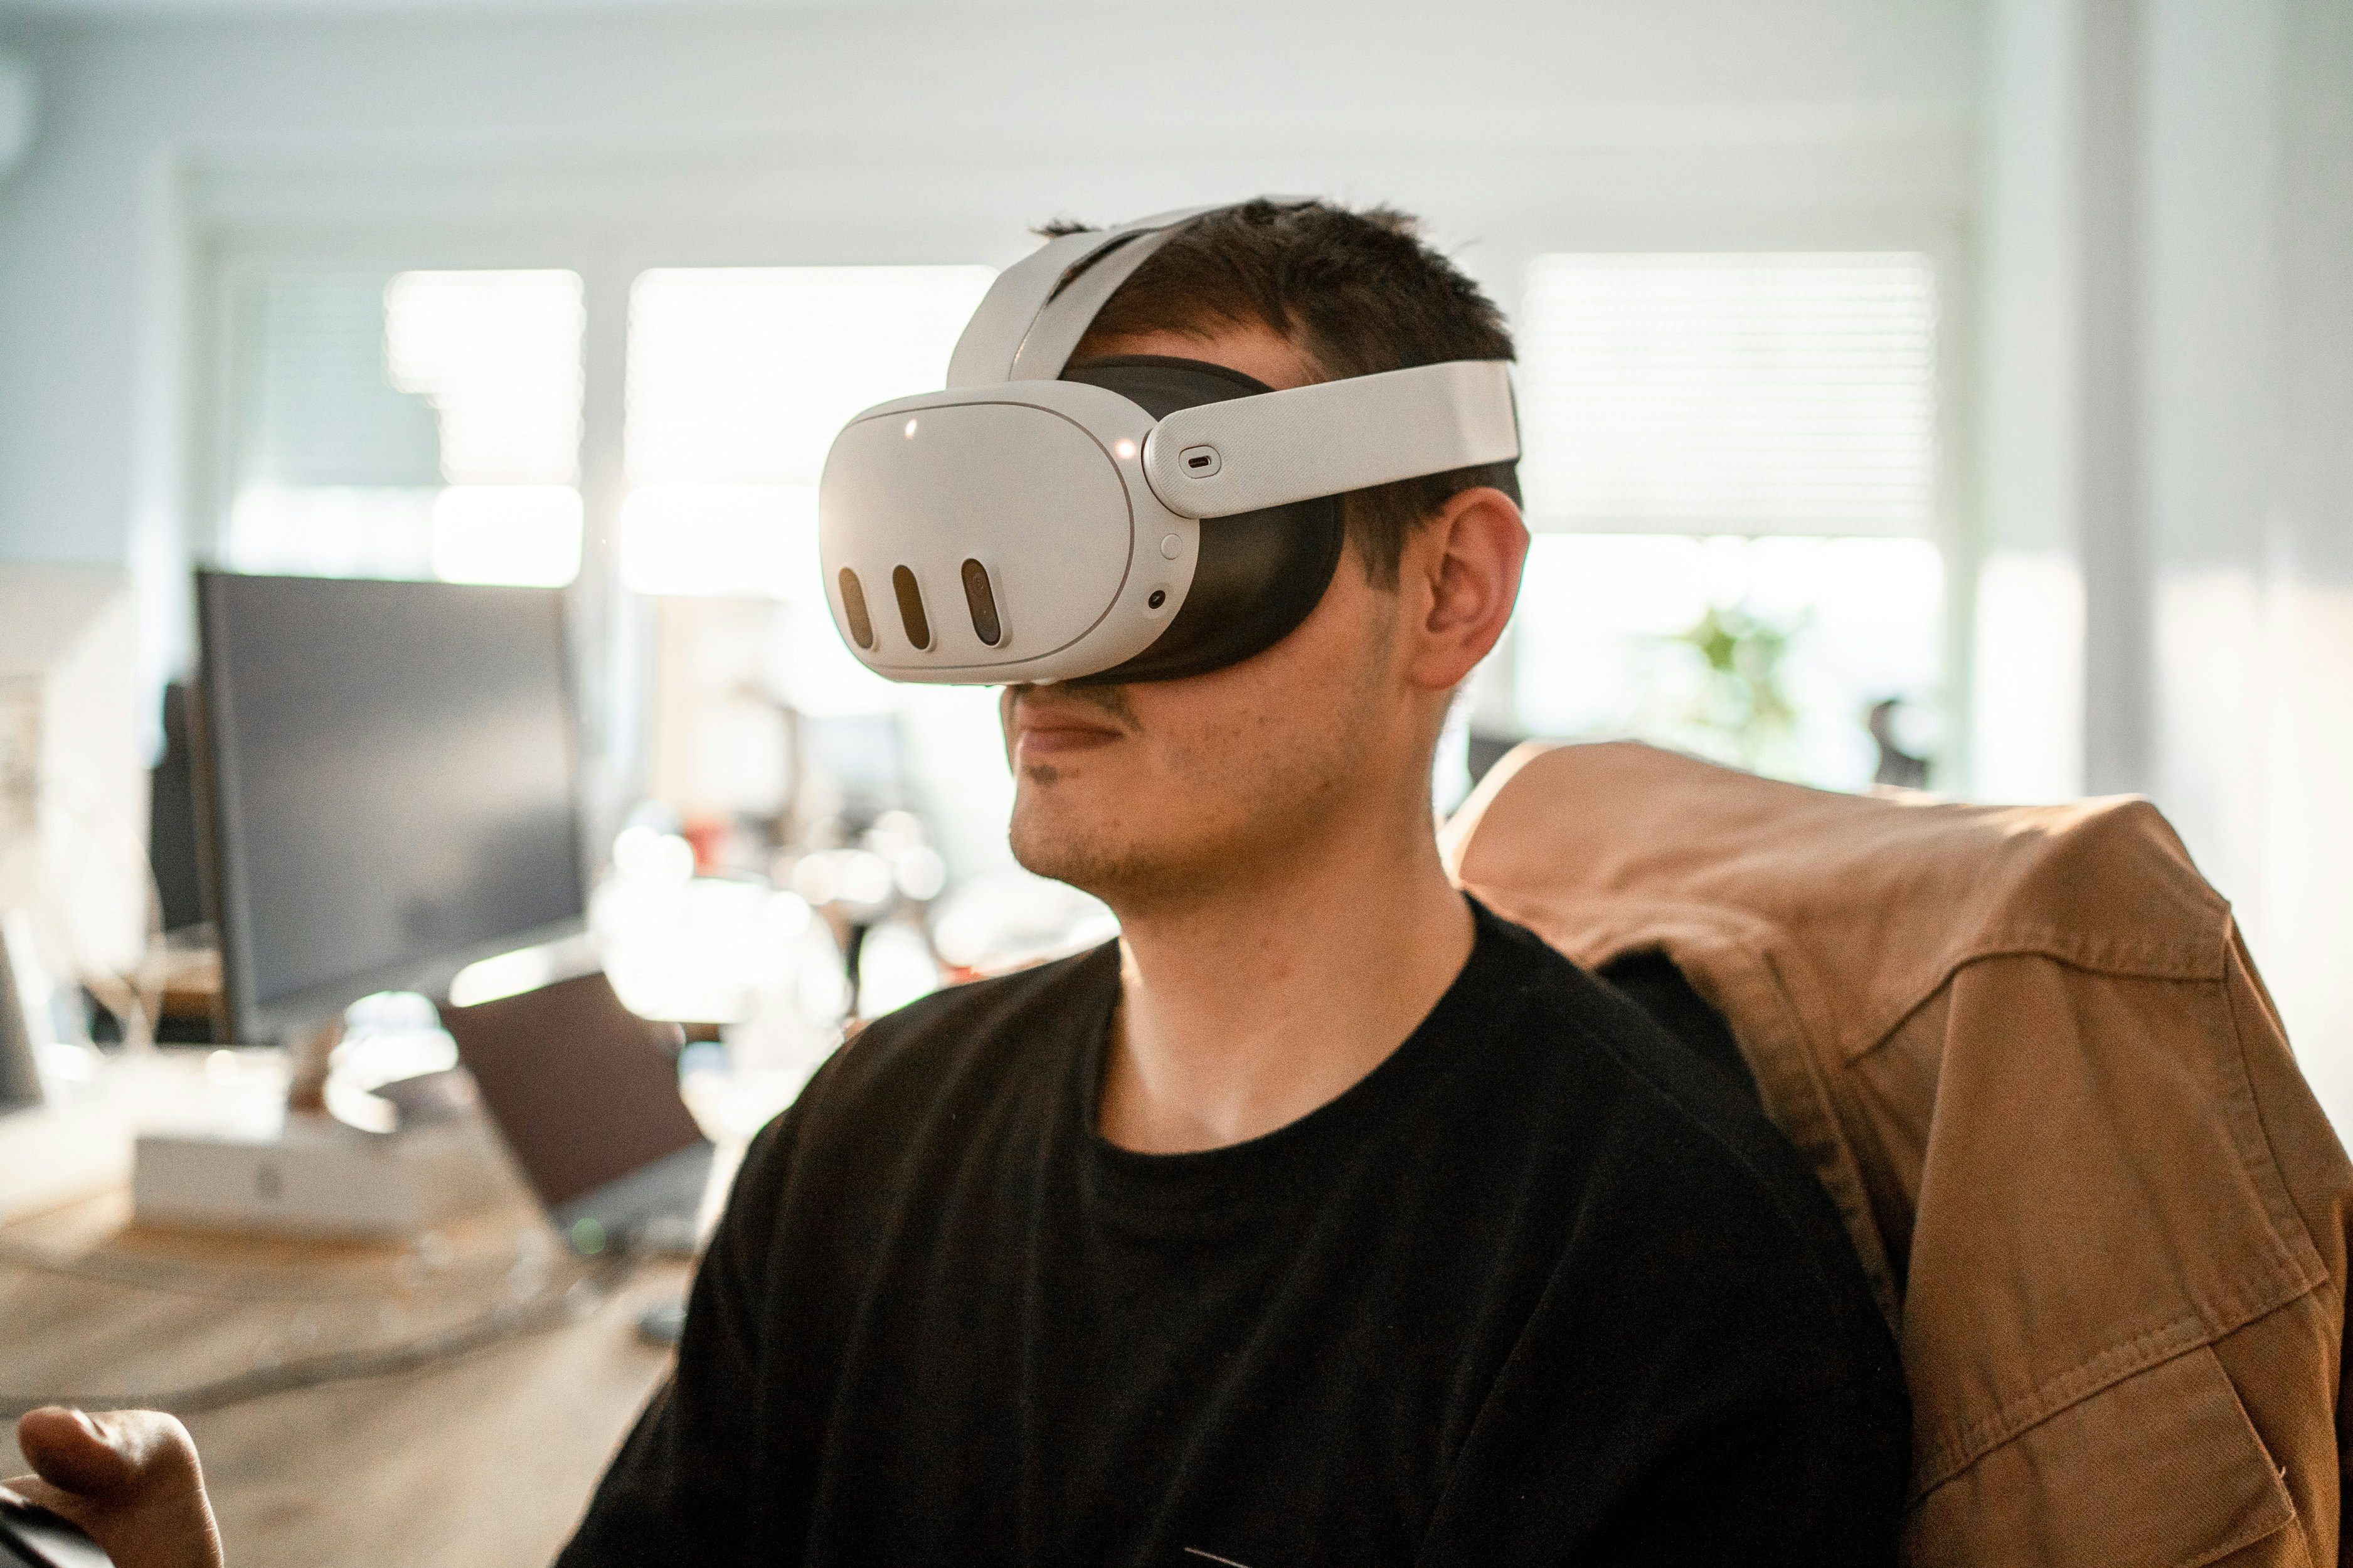
\includegraphics[width=0.9\textwidth]{images/quest3_example.jpg}
      \caption{Oculus Quest 3 VR-Headset}
      \source{https://unsplash.com/de/fotos/ein-mann-der-auf-einem-stuhl-sitzt-und-eine-virtuelle-brille-tragt-AZ-ND5uJ4S4}
      \label{fig:oculus-quest-3}
    \end{figure}

    Jedoch sind nicht alle VR-Headsets für AR geeignet.
    Die meisten VR-Headsets besitzen keine Kamera, um die reale Welt aufzunehmen und dem Nutzer wiederzugeben.
    Nur Headsets wie bspw. die Oculus Quest 3, welche in Abbildung \ref{fig:oculus-quest-3} dargestellt ist, oder die Apple Vision Pro besitzen eine Kamera nach außen, um die reale Welt aufzunehmen und so AR zu ermöglichen.
    
    Durch all diese Technik, können die neusten VR-Headsets eine sehr hohe Immersion und Qualität für Anwendungen in AR bieten.
    Doch für lange Anwendungszeiten und die Verwendung in der Öffentlichkeit sind sie meist zu groß und schwer.

   

    \subsubsection{Smart-Glasses}

    Smart-Glasses sind Brillen, die digitale Informationen in das Sichtfeld des Nutzers einblenden.
    Grundsätzlich sind auch sie HMDs, jedoch werden sie aufgrund ihrer 
    Sie stellen Informationen auf einer semitransparenten Fläche dar, sodass der Nutzer weiterhin die reale Welt sehen kann.

    Da sie fast aussehen wie normale Brillen die unauffälligste Art von AR-Anzeigegeräten.
    Dadurch sind sie auch in der Öffentlichkeit unauffällig zu tragen und können so potentiell auch im Alltag genutzt werden.
    Zudem sind sie, vor allem über einen längeren Zeitraum, meist deutlich leichter und angenehmer zu tragen als HMDs.


  \subsection{Hand-Held-Devices}

  Hand-Held-Devices sind Geräte, die ein Nutzer in der Hand hält.
  Diese Kategorie besteht heutzutage hauptsächlich aus Smartphones und Tablets, da die meisten dieser Geräte über eine Kamera und einen Bildschirm verfügen, können sie fast alle für die Darstellung von AR-Inhalten genutzt werden.
  Das Smartphone oder Tablet ist dabei wie ein Fenster in die digitale Welt, durch das der Nutzer die erweiterte Realität sehen kann.

  Die Immersion ist bei diesem Anzeigegerät jedoch relativ gering, da der Nutzer immer die reale Welt sieht und das Smartphone oder Tablet nur ein kleines Fenster in die digitale Welt ist.
  Allein durch die Entfernung der Geräte vom den Augen der Nutzer können sie nur ein vergleichsweise kleines Sichtfeld abdecken.
  Jedoch ist die Nutzung von Smartphones für AR sehr weit verbreitet, da fast jeder ein Smartphone besitzt und so keine zusätzliche Hardware benötigt wird.

  Auch können Smartphones als Displays für HMDs genutzt werden, um so die Rechenleistung des Smartphones zu nutzen und die Immersion zu steigern.
  Dabei ist jedoch meist die Kamera des Smartphones nicht mehr nutzbar, wodurch normalerweise nur VR möglich ist.
  Zudem ist die Pixeldichte von Smartphones meist geringer als bei speziellen AR-Anzeigegeräten, was die Immersion und Nutzererfahrung verschlechtern kann, da das Display sehr nah an den Augen des Nutzers ist.

  

  \subsection{Spatial Displays}